\subsection[Standortarten]{Standortarten
 \\ \textnormal{\small{\textit {Verfasst von Victor Schwartz}}}}

Betrachtet man den Titel dieser Arbeit „Location Based Services“ (Standort bezogene Dienste), wird schnell klar aus welchen Bestandteilen sich LBS zusammensetzt: der eigene Standort und ein Dienst, der diesen nutzt. Dieses Kapitel beschäftigt sich damit, wie ein Standort beschrieben werden kann.
\\Als einleitendes Beispiel kann man sich vorstellen, man steht mitten in einer Stadt wie Mannheim. Für einen selbst ist klar wo der eigene Standort ist. Will man diesen einem Freund mitteilen, kann dies schwierig sein. Deshalb gibt es definierte Arten seinen Standort bis auf wenige Zentimeter genau zu beschreiben. Dieses Kapitel ist in mehrere Abschnitte unterteilt. Jeder Abschnitt erläutert eine mögliche Beschreibung des eigenen Standortes.
Zu beachten ist an dieser Stelle, dass es sich hierbei nicht um alle Möglichkeiten handelt einen Standort zu beschreiben. Es ist immer möglich eine individuelle Beschreibung des eigenen Standortes anzugeben. 

%\textbf{Standortbeschreibung anhand der Sterne}\\
\textbf{Standortbeschreibung mit einem Kompass}
\\Dieser Abschnitt beschreibt wie man mit Hilfe eines Kompasses seine Position bestimmen bzw. angeben kann. Hierfür wird erst vorgestellt wie ein Kompass funktioniert und welche Voraussetzungen zur Standortbestimmung gegeben sein müssen.
\\Bei einem Kompass handelt es sich um ein Gerät, dessen Aufgabe es ist, in die Richtung des Nordpol zu zeigen. Dieses Ziel wird durch das Erdmagnetfeld erreicht.


\begin{figure}[ht]
  \centering
    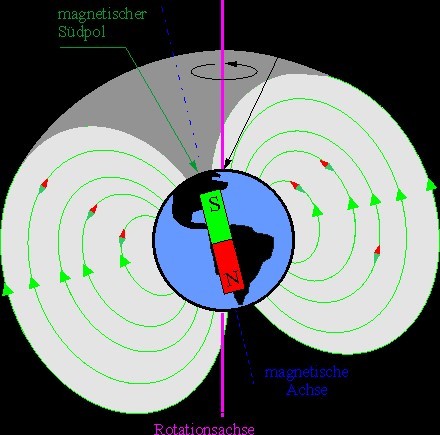
\includegraphics[width=0.50\textwidth]{ref/images/magnetfeld.jpg}
   \caption{Magnetfeld der Erde}
  \label{fig:Magnetfeld}
  \cite{Magnetfeld}
\end{figure}



 
Das Erdmagnetfeld ist in Abbildung \ref{fig:Magnetfeld} zu sehen. Durch dieses Feld ist die komplette Erdkugel magnetisiert. In der Nähe des geografischen Südpols liegt der magnetische Nordpol. Umgekehrtes gilt für den geografischen und magnetischen Nord- bzw. Südpol.
Mit Hilfe eines magnetisierten Metallstücks kann dieses Feld genutzt werden. Meist handelt es sich dabei um  eine Nadel,  die dann in Richtung Norden zeigt.


\begin{figure}[h]
  \centering
    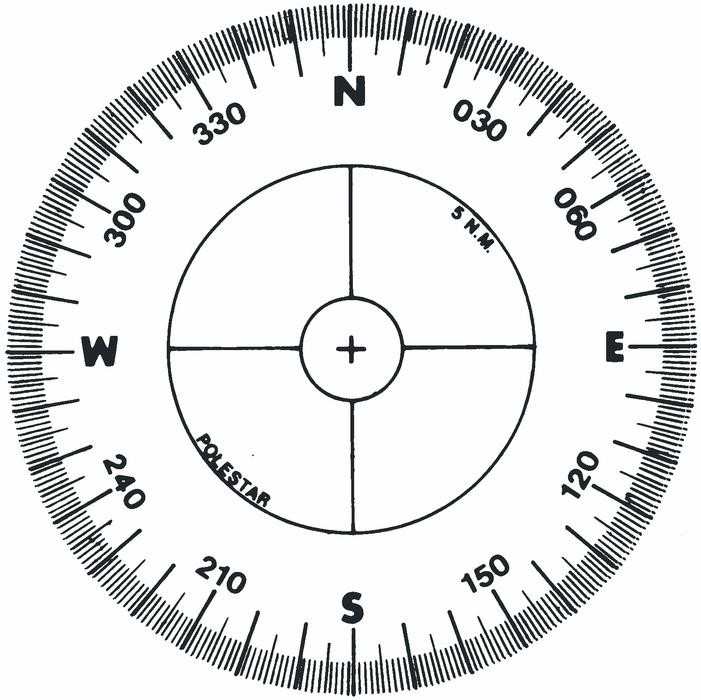
\includegraphics[width=0.50\textwidth]{ref/images/kompassrose.jpg}
   \caption{Kompassrose mit Gradzahlen}
  \label{fig:Kompassrose}
   \cite{Kompassrose}
\end{figure}


 
Bei einem Kompass kommt neben der Nadel auch eine Kompassrose  (siehe Abbildung \ref{fig:Kompassrose}) zum Einsatz. Mit Hilfe dieser Rose lässt sich eine Gradzahl ablesen. Sie orientiert sich immer am Abstand von der angezeigten Richtung des Norpols. Diese Gradzahl kann für die Beschreibung des eigenen Standort genutzt werden. Wie dieses Verfahren funktioniert, wird im nächsten Abschnitt erklärt.

\underbar{Standortbeschreibung mit zwei Fixpunkten}
\\Möchte man seinen geografischen Standpunkt jemandem mitteilen oder sich diesen notieren, muss man ihn beschreiben. Hat man dafür nur einen Kompass zur Verfügung, kann man sich zwei Fixpunkte zur Hilfe nehmen um den eigenen Standort zu bestimmen.
Anhand eines Beispiels soll dieses Verfahren erklärt werden. 
\\Befindet man sich auf einem Boot in der Nähe der Küste und möchte den Standort mit einem Kompass bestimmen, so sucht man sich zwei gut sichtbare Punkte an der Küste, dies können beispielsweise Leuchttürme oder eindeutig identifizierbare Felswände sein. Nun fixiert man den ersten Punkt mit dem Kompass und liest die exakte Grad Zahl auf der Kompassrose ab. Mit Hilfe der Angabe von Gradzahl und dem erstem Fixpunkt, kann der eigene Standort auf eine Linie differenziert werden. Um nun den Standort auf einen Punkt zu differenzieren fixiert man mit dem Kompass den zweiten Fixpunkt und liest ebenfalls die Grad Zahl ab. Zeichnet man diese Informationen in eine Karte ergibt sich ein Schnittpunkt von zwei Geraden. An dieser Stelle befindet man sich. Die Beschreibung des eigenen Standortes könnte beispielsweise wie folgt aussehen:
\\270 Grad von Leuchtturm X
\\250 Grad von Gebäude Y
\\Der Vorteil dieses Verfahren ist: Es kann überall angewendet werden, wo es Fixpunkte gibt.
Nachteile dieser Methode sind: Es wird keine Höhe angegeben und es kann eine große Ungenauigkeit beim Ablesen des Kompasses entstehen.

\textbf{Standortbeschreibung mittels einer Adresse}
\\Im Gegensatz zur eben vorgestellten Standortbeschreibung, ist folgende wesentlich bekannter und gebräuchlicher. Es handelt sich um die Anschrift bzw. Adresse. Bei dieser Beschreibung wird kein exakter Standort angeben, sondern ein Haushalt. Dies geschieht über einen Namen, eine Straße mit Hausnummer und die Angabe einer Stadt, welche konkretisiert über die Postleitzahl angeben wird.  
Eine Adresse kann in Deutschland beispielsweise wie folgt aus:
\\Max Mustermann 
\\Coblitzalle 53
\\12345 Mannheim
\\Im folgenden Abschnitt werden die Bestandteile einer Adresse detailliert beschrieben.
\\\underbar{3. Zeile: Postleitzahl und Stadtname}
\\Die letzte Zeile der Adresse enthält den Namen einer Stadt, sowie eine Postleitzahl. Bei der Angabe der Stadt handelt es sich um die gröbste Angabe innerhalb der Adresse. Mit Hilfe des Stadtnamens soll eine erste Orientierung innerhalb Deutschlands ermöglicht werden. Es handelt sich nicht nur um Großstädte wie Berlin, Frankfurt, Hamburg etc. sondern alle Gemeinden, welche den Titel Stadt tragen .
Da manche Stadtnamen mehrfach vorkommen oder die Angabe zu ungenau ist, wird der Stadname mit der Postleitzahl (PLZ) definiert bzw. konkretisiert. Allein für die Stadt Mannheim gibt es über 15 verschieden Postleitzahlen. Diese sind teilweise jedem Stadtteil zugeordnet. In Abbildung \ref{fig:Postleitzahlgebiete} ist eine Karte mit den Postleitzahlgebieten von Deutschland zu sehen.



\begin{figure}
  \centering
    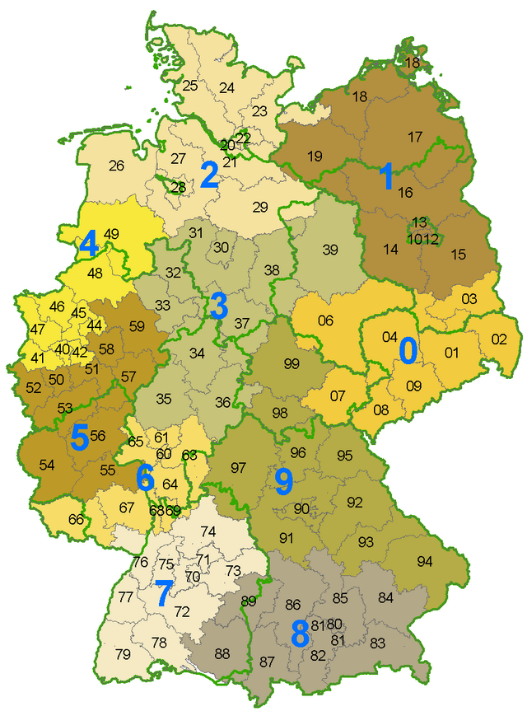
\includegraphics[width=0.50\textwidth]{ref/images/plzgebiete.png}
   \caption{Postleitzahlgebiete in Deutschland}
  \label{fig:Postleitzahlgebiete}
   \cite{PLZGebiete}
\end{figure}


\underbar{1 und 2. Zeile: Vor- und Nachname, Straßenname und Hausnummer}
\\Da die Angabe von einer Stadt und der dazugehörigen PLZ das Gebiet noch nicht weit genug einschränkt um einzelne Häuser bzw. Haushalte zu identifizieren, wird ein Straßenname angegeben.
Die europäischen Straßennamen sind meist mit Namenwörtern angeben.
Einige Beispiele hierfür sind:
\\-	Lindenstraße
\\-	Schillerstraße
\\-	Hauptstraße
\\Um ein Haus innerhalb einer Straße exakt definieren zu können bedient man sich einer Nummerierung, den sogenannten Hausnummern. Jedes Haus hat eine eigene Hausnummer. 
Da es häufig vorkommt, dass in einem Haus mehrere Parteien wohnen, wird neben den beschriebenen Bestandteilen einer Adresse noch ein Empfänger mit Vor- und Nachname oder nur Nachnahme angegeben.
Diese Beschreibung findet auf der ganzen Welt Anwendung, allerdings nicht immer in diesem Format. Das beschrieben Format trifft größtenteils in Europa zu. 

\underbar{Verwendung von Adressen}
\\Die vorgestellte Beschreibung des eigenen Standortes mithilfe einer Adresse ist besonders wichtig für Brief- und Paketversandorganisationen. In Deutschland wurden in den letzten Jahren hauptsächlich mit der Deutschen Post AG Briefe verschickt. Sie ist darauf angewiesen, dass auf jedem Paket und Brief die Adresse im beschriebenen Format angegeben ist, damit eine Zustellung erfolgen kann.
Desweiteren hat die Adresse mit der Entwicklung von Navigationsgeräten und somit für LBS stark an Bedeutung dazu gewonnen. Im Jahr 2014 besaßen ca. 48 Prozent der deutschen Haushalte ein Navigationsgerät. \cite{Navi} Dort wird das Ziel hauptsächlich als Adresse angegeben. 
Auch im Alltag wird die Adresse meist zur Beschreibung des eigenen Standortes verwendet. Möchte man Freunde zu sich einladen, gibt man meist die Adresse an und mit einem Navigationsgerät oder einer Karte kann der Haushalt gefunden werden.
\\Vergleicht man eine Adresse mit der Standortbeschreibung des letzten Kapitels über einen Kompass, ist zu erkennen, dass man sich einen groben Überblick über den Standort mit Adresse viel leichter verschaffen kann. Die Koordinaten eines Kompasses kann man nur mit entsprechendem Fachwissen deuten. 
\\Als Nachteile zählen die Genauigkeit und Abdeckung der Erde mit Adressen. Die Genauigkeit des eigenen Standortes kann mit einer Adresse nicht exakt angegeben werden. Während bei einer kleinen Einzimmerwohnung der Standort auf wenige Meter genau angegeben werden kann, kann sich dies auf mehrere Kilometer ausweiten, wenn die Adresse zu einem großen Anwesen gehört. Für manche Location Based Sevices ist es wichtig, dass diese auch in nicht besiedelten Gebieten verwendet werden können. Hierzu zählen beispielsweise LBS zum Wandern und Radfahren. Hierfür eignet sich die Angabe des eigenen Standortes mit einer Adresse nicht, da ein Standort nur auf der Minderheit der Erde mit einer Adresse angegeben werden kann. 
Im nächsten Abschnitt wird die Beschreibung des Standortes mithilfe von Längen- und Breitengraden erläutert.

\textbf{Standortbeschreibung mit Längen- und Breitengraden}


\begin{figure}
  \centering
    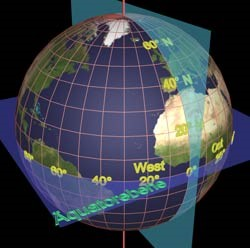
\includegraphics[width=0.50\textwidth]{ref/images/grade.jpg}
   \caption{Längen- und Breitengrade der Erde}
  \label{fig:Grade der Erde}
   \cite{Grade}
\end{figure}



Dieser Abschnitt erläutert die Standortbeschreibung mittels Längen- und Breitengraden.
Hierfür kann man sich ein zweidimensionales Koordinatensystem vorstellen, welches den Nullpunkt im Zentrum besitz., Dieses „Netz“ legt man bildlich gesprochen über den Globus. So kann für jeden Ort auf dem Globus eine exakte Beschreibung stattfinden. 
\\\underline{Grundlagen für diese Standortbeschreibung}
\\Beim Globus handelt es sich annähernd um eine Kugel. Diese Kugel dreht sich in ca. 24 Stunden um ihre eigene Achse. Die Achse kann man sich als gedachte Gerade vorstellen, welche an der untersten Stelle, dem Südpol einsticht und am obersten Punkt, dem Nordpol, wieder austritt. Stellt man sich nun die Achse als Strecke vom Nord- zum Südpol vor und halbiert diese, befindet man sich im ungefähren Mittelpunkt des Globus. Spannt man auf der Höhe der halbierten Achse einen Kreis um den Globus, so befindet man sich an der dicksten Stelle, dem Äquator. Dieser befindet sich im rechten Winkel zur Achse.
\\\underline{Breitengrade}
\\Nachdem der Äquator im letzten Abschnitt definiert wurde, wird nun erklärt was Breitengrade sind. Um den gesamten Globus mit Graden zu beschreiben, hat man sich dazu entschieden den Globus am Äquator in eine nördliche und eine südliche Halbkugel aufzuteilen. Der gesamte Globus ist in 180 Breitengrade aufgeteilt. Beim Äquator handelt es sich um den 0. Grad. In Abhängigkeit dieses Grades wird der Standort auf einem Breitengrad angegeben. Es gibt jeweils 90 Grade in die nördliche und südliche Richtung. Mithilfe dieser Angabe kann man seinen Standort auf eine Linie um den Globus beschränken. Die Stadt Mannheim beispielsweise liegt auf der Linie welche im 49 Grad Winkel zum Äquator steht auf der nördlichen Halbkugel. Im Vergleich hierzu liegt Sydney im 33 Grad Winkel zum Äquator auf der südlichen Halbkugel.
Damit der eigene Standort nicht nur einer Linie beschrieben werden kann, welche eine Länge von 40.075km haben kann, gibt es Längengrade. Diese beiden Graden schneiden sich bei der Standortbeschreibung in einem Punkt und geben den Standort exakt an.
\\\underline{Längengrade}
\\Ähnlich wie bei Breitengraden handelt es sich bei Längengraden um gedachte Linien um den Globus. Längengrade stehen  senkrecht zum Äquator und nicht parallel wie die Breitengrade. Bei diesen Graden ist zu beachten, dass sie immer den gleichen Umfang besitzen. Um den kompletten Globus abzudecken gibt es 360 Längengrade. Diese wurden aufgeteilt in westliche und östliche Grade mit jeweils 180 Grad. Für Längengrade gibt es keinen gegebenen Nullpunkt wie den Äquator. 1883 wurde sich darauf geeinigt den Nullmeridian (0. Längengrad) durch eine Sternenwarte im englischen Greenwich laufen zu lassen. Seit dieser Einigung wird der Längengrad in Abhängigkeit des Winkels zur Stadt Greenwich angegeben. 
Für die Beispiele des letzten Abschnitts heißt das: Die Stadt Mannheim liegt auf dem 8. Längengrad östlich von Greenwich und Sydney auf dem 151. Grad östlich von Greenwich.
\\\underline{Genauigkeit der Längen- und Breitengrade}
\\Der Umfang des Globus beträgt ca. 40.000 km. Teilt man diesen nun durch 360 Längengrade erhält man einen Abstand von 111km zwischen zwei Längengraden. Das bedeutet, wenn der Längengrad lediglich mit einer Gradzahl angegeben ist, handelt es sich um eine Strecke von 111km auf dem der Standort liegen kann. Daher teilt man entweder ein Grad in 60 Minuten und eine Minute in 60 Sekunden, was eine Strecke von 30m entspricht oder man gibt zu einer Grad Zahl Dezimalstellen an. Bei der Angabe von 5 Dezimalstellen beträgt die Genauigkeit ca. 1 Meter.
Durch die Krümmung der Erde, lässt sich diese Rechnung nicht auf Breitengrade übertragen.

Eine vollständige Angabe des Standortes könnte wie folgt aussehen:
\\49 Grad 29 Minuten N, 8 Grad 28 Minuten O  
\\49.487459 N, 8.466039 O 
\\Ein Nachteil dieser Standortbeschreibung ist, dass man sich nicht direkt ein Bild von der Position machen kann. Nur die wenigsten Menschen kennen sich so gut mit Koordinaten aus um sich direkt den Standort auf einer Karte vorzustellen.
\\Die Vorteile dieser Beschreibung liegen in der Abdeckung. Der gesamte Globus kann mit diesem Verfahren beschrieben werden. Es gibt keinen Ort, der nicht mit Längen- und Breitengraden beschrieben werden kann. Dies ist ein Grund dafür, weshalb Längen- und Breitengrade für LBS hauptsächlich genutzt werden.
\cite{QuelleGrade}


%Adresse + PLZ, analoge Karte, Länge+Breit, 3D-Position, indoor (WLAN Blue)